\documentclass[10pt,a4paper]{article}
\usepackage[utf8]{inputenc}
\usepackage{amsmath}
\usepackage{amsfonts}
\usepackage{amssymb}
\usepackage{graphicx}
\usepackage{caption}
\usepackage{sidecap}
\usepackage{framed}
\title{Report Multi-agent Systems Module II}
\author{Tom Jacobs (s0214835), Thomas Uyttendaele (s0215028)}
\begin{document}
\maketitle
\part{}
\section{Value iteration in MDPs}
The different implementations of Value Iteration have been verified using the $Q^{*}$ provided for the \emph{loadunload} problem. They match exactly within the accuracy of the reference matrix.
\paragraph{Performance statistics}\hfill

\begin{table}[!h]
\centering
\begin{tabular}{ c || c | c || c | c}
Problem & Mean Old & Mean New & Std Dev Old & Std Dev New \\
\hline
loadunload & 3.744e-02 & 3.213e-02 & 1.035e-03 & 1.305e-03\\
hallway & 7.463e-01 & 7.167e-01 & 1.0582e-02 & 9.933e-03\\
hallway2 & 1.167e+00 & 1.115e+00 & 1.024e-02 & 9.640e-03 \\
trc & 1.408e+01 & 1.418e+01 & 1.850e-01 & 2.250e-01\\
\end{tabular}
\caption{Value Iteration runtime statistics for both algorithms}
\label{table:vi}
\end{table}

The algorithm for \emph{Value Iteration} presented in the slides was implemented with a few minor modifications for performance reasons. 
Looping is first done over actions and then nested the different states. To exploit the sparsity of some of the matrices the Matlab \emph{find()} function is used.

To optimize the calculation of the $Q^{*}$ matrices a second implementation was done where the fetching of the non-zero elements from sparse matrices is done up front. 
The average running time and standard deviation of running times in seconds for \emph{Value Iteration} can be found in table \ref{table:vi}.
Here the new algorithm is the modified version with fetching before the actual loops.
\begin{framed}
\textit{note: for all timing results presented in this report the first value is removed before processing, as it is usually an outlier due to initialization and caching delays.}
\end{framed}
\begin{SCfigure}
\vspace{-20pt}
\hspace{-30pt}
\centering
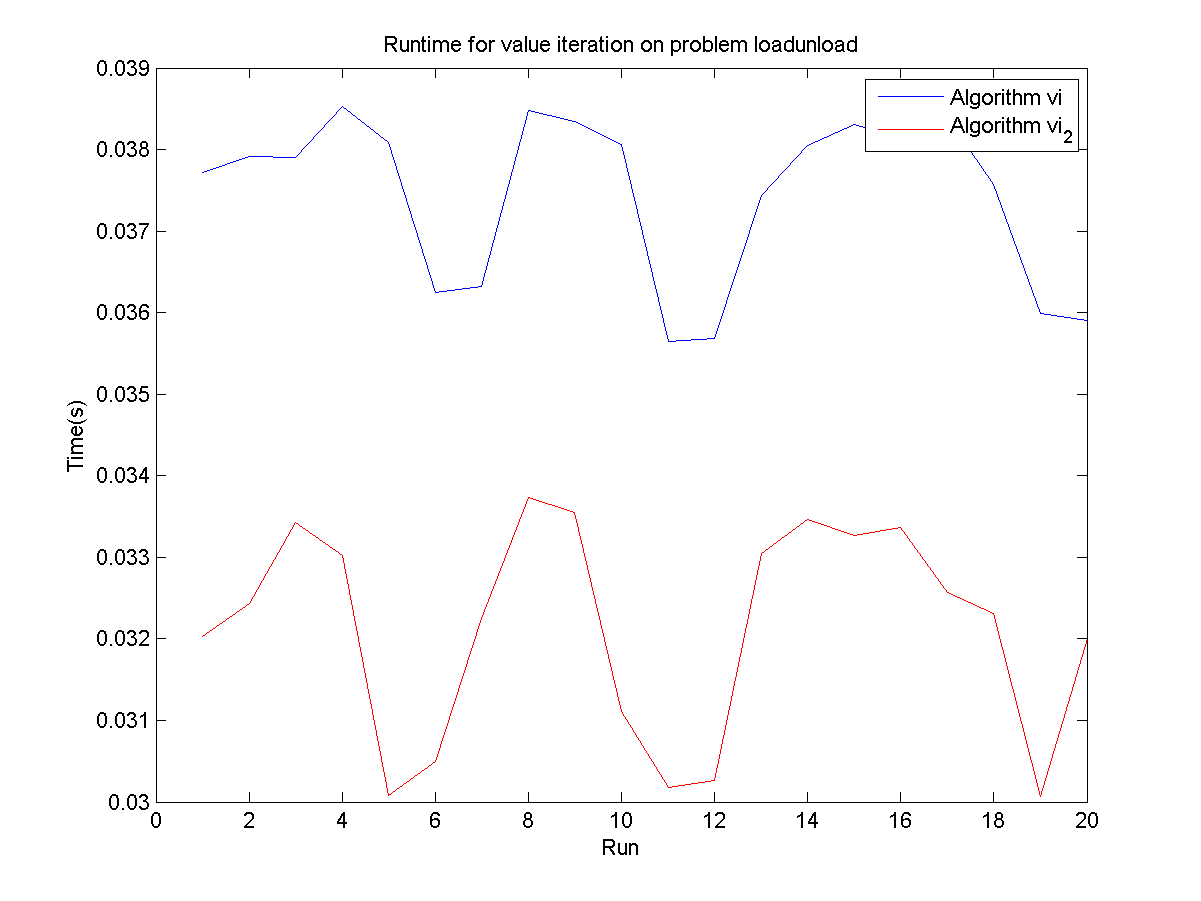
\includegraphics[width=0.8\textwidth]{Timings/loadunload/timings_vi.png}
\hspace{-30pt}
\caption{The loadunload problem}
\label{fig:vi_loadunload}
\vspace{-20pt}
\end{SCfigure}

\begin{SCfigure}
\vspace{-20pt}
\hspace{-30pt}
\centering
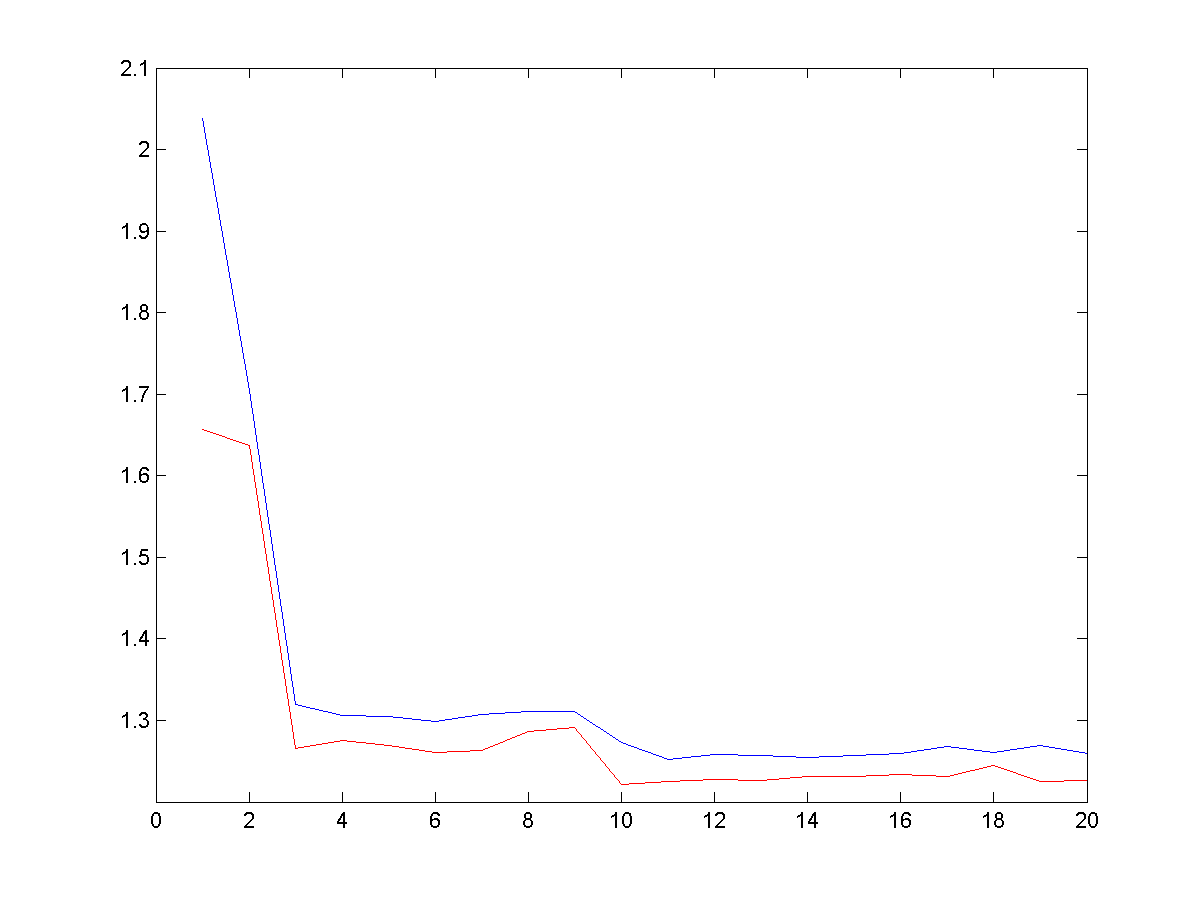
\includegraphics[width=0.8\textwidth]{Timings/hallway/timings_vi.png}
\caption{The hallway problem}
\hspace{-30pt}
\label{fig:vi_hallway}
\vspace{-20pt}
\end{SCfigure}
        
\begin{SCfigure}
\vspace{-20pt}
\hspace{-30pt}
\centering
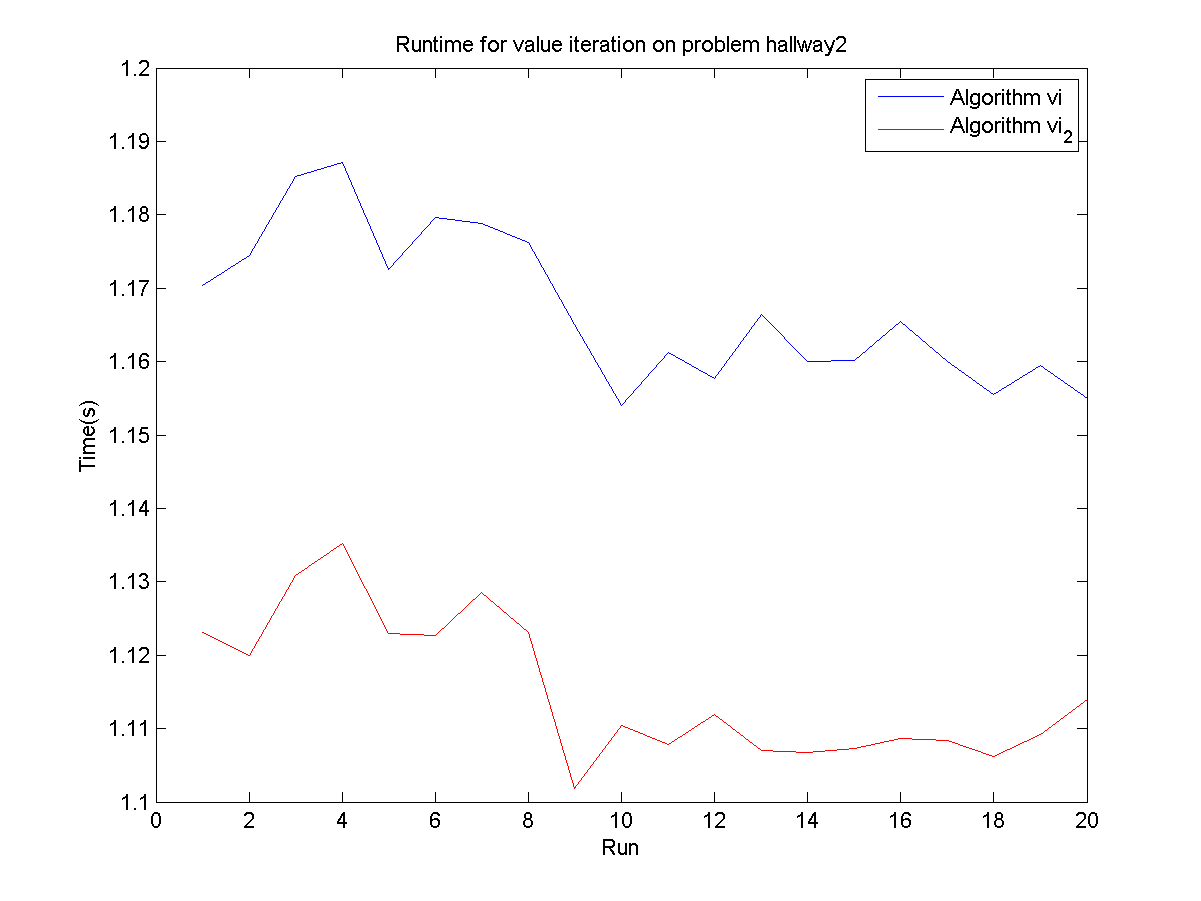
\includegraphics[width=0.8\textwidth]{Timings/hallway2/timings_vi.png}
\caption{The hallway2 problem}
\hspace{-30pt}
\label{fig:vi_hallway2}
\vspace{-20pt}
\end{SCfigure}
        
\begin{SCfigure}
\vspace{-20pt}
\hspace{-30pt}
\centering
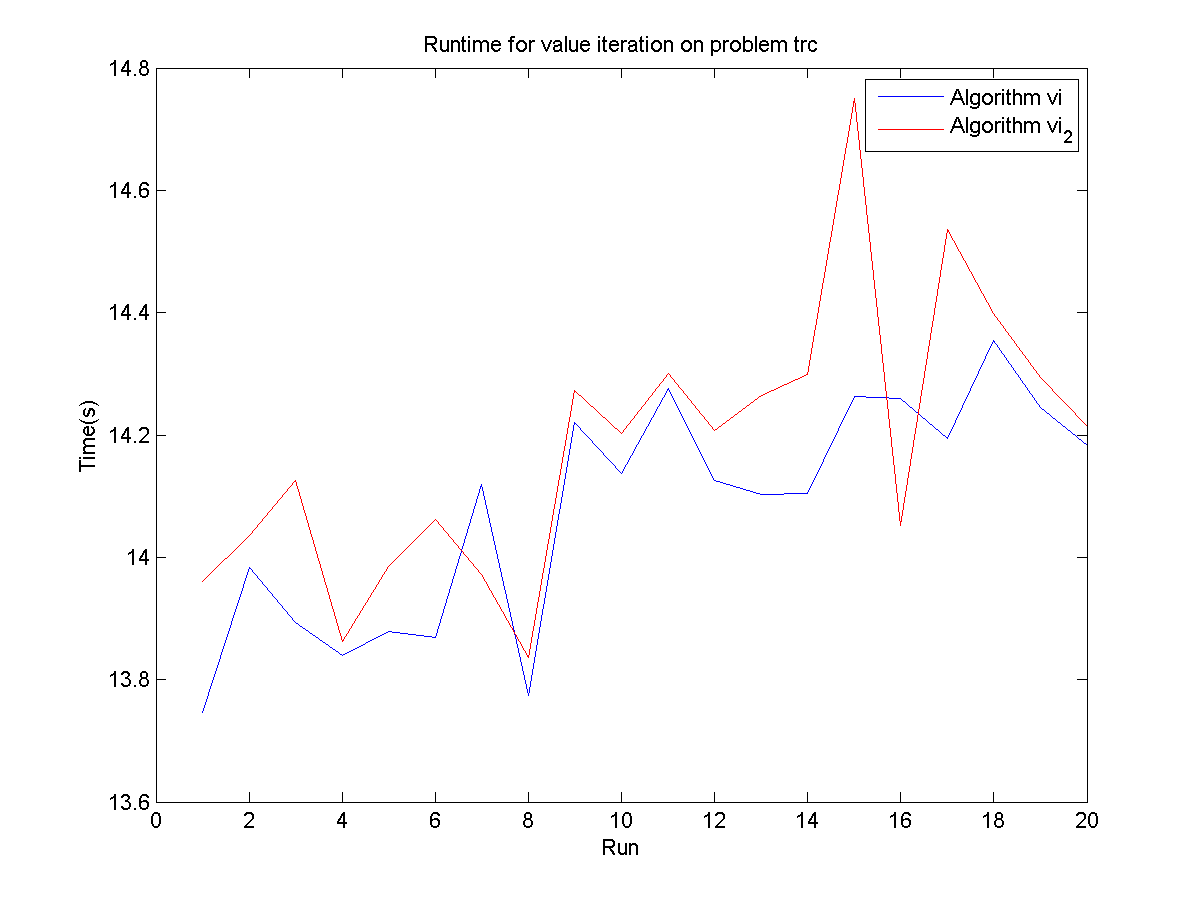
\includegraphics[width=0.8\textwidth]{Timings/trc/timings_vi.png}
\hspace{-30pt}
\caption{The trc problem}
\label{fig:vi_trc}
\vspace{-20pt}
\end{SCfigure}

The average sums of discounted rewards and relevant standard deviations (between parenthesis) have been visualised in \ref{table:rewards}. They are the result of 100 runs with a horizon of 100 steps.

\begin{table}
\centering
\begin{tabular}{ c || c | c | c }
\hfill & Fully Observable & MLS & $Q_{MDP}$\\
\hline
hallway & 7.463e-01 & 7.167e-01 & 1.0582e-02\\
hallway2 & 1.167e+00 & 1.115e+00 & 1.024e-02\\
trc & 1.408e+01 & 1.418e+01 & 1.850e-01\\
\end{tabular}
\caption{Value Iteration runtime statistics for both algorithms}
\label{table:rewards}
\end{table}
 
%%Rewards : horizon 100, 100 iterations.

\section{Partially observable environments: heuristic methods}

\section{Partially observable environments: point-based methods}

\part{}
\section{Multiagent planning under uncertainty}
\end{document}